\section{مجموعه‌های فازی}
 \subsection{مجموعه‌های کلاسیک}
پیش از آنکه به توضیح مجموعه‌های فازی بپردازیم، نیاز است تا مروری بر مجموعه‌های کلاسیک داشته باشیم. همه‌ی ما کم و بیش با مفهموم مجموعه آشنا هستیم. به عنوان مثال مجموعه‌ای از دانشجویان یک رشته، مجموعه‌ای از اعداد بزرگ‌تر از صفر و... نمونه‌ای از مجموعه‌ها هستند. مجموعه‌ها گروهی از اشیاء متمایز هستند. به اشیاء درون هر مجموعه، اعضاء و یا عناصر آن مجموعه گفته می‌شود. \\
در ریاضیات مجموعه را با حروف بزرگ 
$\lr{A,B,C,...}$
 و اعضای مجموعه را با حروف کوچک 
$\lr{a,b,c,...} $
  نمایش می‌دهند. همچنین عضویت یک شیء در مجموعه با نماد 
$\in$
 و عدم عضویت با نماد
 $\notin$
 نمایش داده می‌شود. 
 \cite{Bojadziev2007}
 \\
مجموعه‌ای را که شامل همه‌ی اشیاء در یک کاربرد مشخص هستند را مجموعه‌ی جهانی 
\LTRfootnote{Universal Set}
یا مرجع گویند. \\
اگر مجموعه‌ی جهانی را با $ U $  نمایش دهیم، آنگاه نمایش مجموعه‌ی $ A $  در این مجموعه‌ی مرجع می‌تواند به دو روش صورت گیرد. در روش اول می‌توان تمامی عناصر موجود در مجموعه را با لیست کردن 
\LTRfootnote{Listing Method}
نمایش داد. به عنوان مثال اگر مجموعه‌ی $ A $ مجموعه‌ی اعداد طبیعی کوچک‌تر از ۵ باشد، می‌توان آن را به صورت زیر نمایش داد:
$$ A=\{1,\ 2,\ 3,\ 4\} $$
و یا می‌توان با استفاده از روش دوم یعنی قانون عضویت
\LTRfootnote{Membership Rule}
بصورت زیر نمایش داد
\cite{Wang1997}:
 $$A= \{ x\ |\ x \in N,\ x < 5\} $$
 روش دوم به این صورت خوانده می‌شود «مجموعه‌ی $ A $، شامل اعضای $ x $ است، به قسمی که  $ x $ها جزو اعداد طبیعی باشند و کوچک‌تر از ۵ باشند».\\
 به صورت کلی تعریف مجموعه‌ها با استفاده از قوانین عضویت به صورت زیر نوشته می‌شود:
\begin{equation}
 A= \{  x \in U\ |\   x\ {\rm meets\ some\ conditions } \}
 \end{equation} 
 در مجموعه‌های کلاسیک عضویت یک شیء تنها دو حالت دارد؛ بدین صورت که شیء $x$ یا متعلق به مجموعه $A$ هست و یا نیست. این مجموعه‌ها را به دلیل آنکه فضای آن با دقت ۱۰۰٪ قابل تشخیص است و عناصر آن دارای ارزش عضویت صفر و یا یک هستند، مجموعه‌های
  \textbf{قطعی}
  نیز می‌گویند. 
\begin{equation}\label{eq:e_classic_setdesc}
\mu_{A}(x)=\left \{ 
	{1 \atop 0}
	\hskip 1cm
   {if \hskip 1cm x \in A, \atop
	if \hskip 1cm x \notin A.} \right.
\end{equation} 
در اینجا
$\mu_{A}(x)$
 تابع عضویت مجموعه‌ی قطعی $A$ می‌باشد. تابع عضویت، تابعی است که ارزش عضویت یک شیء را در یک مجموعه، مشخص می‌کند. طبق آنچه در رابطه
 \ref{eq:e_classic_setdesc}
 آمده است، تابع عضویت مجموعه‌های قطعی، تنها دو مقدار یک و یا صفر را برای مشخص کردن عضویت و یا عدم عضویت یک شیء در مجموعه، بازمی‌گرداند. تابع عضویت مجموعه‌ی جهانی همواره مقدار یک (۱) را بازمی‌گرداند. همچنین اگر مجموعه‌ای دارای هیچ عضوی نباشد، آن مجموعه‌ را تهی
 \LTRfootnote{Empty Set}
 می‌نامند و با علامت $\varnothing$ نمایش داده می‌شود. طبیعی است که  تابع عضویت مجموعه‌ی تهی نیز همواره مقدار صفر (۰) را بازمی‌گرداند. مجموعه‌ی تهی زیرمجموعه‌ی هر مجموعه‌ای است.
 \cite{Lee2005}
 \\
فرض کنید دو مجموعه‌ی $ A $ و $ B  $ در مجموعه‌ی مرجع $ U $ وجود دارد.  در جدول   
\ref{table:t_classic_rel}
\textbf{روابط بین مجموعه‌های کلاسیک} 
 همراه با توضیح آورده شده است:
\begin{table}[!htbp]
\begin{center}
	{\footnotesize
 \begin{tabular}{r c c r} \hline
عنوان & نماد &  مثال & توضیح  
\\\hline 
%**********
زیر مجموعه  &
$\subseteq$ &
$A \subseteq B$ &
همه‌ی اعضای $A$ در $B$ نیز هست و یا دو مجموعه با یکدیگر مساوی هستند.
\\
%*********
زیر مجموعه سره &
$\subset$ &
 $A \subset B$ &
همه‌ی اعضای $A$ در $B$ نیز هست. ولی حداقل یک عضو در $B$ هست که در $A$ نیست.
\\
%**********
مساوی &
$=$ &
$A = B$ &
همه‌ی اعضای $A$ در $B$ نیز هست و همه‌ی اعضای $B$ نیز در $A$ هست.
\\\hline
 %**********
 \end{tabular}
 \caption{روابط بین مجموعه‌های کلاسیک}
 \label{table:t_classic_rel}
}
\end{center}
\end{table}\\
همچنین در جدول
\ref{table:t_classic_op}
\textbf{عملیات بر روی مجموعه‌های کلاسیک} 
همراه با تعاریف هریک از آنها آورده شده‌ است:
\begin{table}[!htbp]
	{\normalsize
	\begin{center}
		\begin{tabular}{r c l} \hline
			عنوان & نماد & تعریف  
			\\\hline 
			%**********
			اجتماع   &
			$\cup$ &
			$A \cup B = \{x\ |\ x \in A\ {\rm or}\ x \in B \}$ 
			\\
			%*********
			اشتراک   &
			$\cap$ &
			$A \cap B = \{x\ |\ x \in A\ {\rm and}\ x \in B \}$ 
			\\	
			%**********
			مکمل &
			$\overline{A}$ &
			$\overline{A} = \{x\ |\ x \notin A{\rm ,}\ x \in U \}$ 
			\\
			%**********
			تفاضل &
			$|$ &
			$A \ |\ B = A\cap \overline{B} = \{x\ |\ x \in A\ {\rm and}\ x \notin B \}$ 
		   \\\hline 
			%**********
		\end{tabular}
		\caption{عملیات بر روی مجموعه‌های کلاسیک}
		\label{table:t_classic_op}
\end{center}
	}
\end{table} \\
 در جدول
\ref{table:t_classic_properties}
\textbf{خواص عملیات بر روی مجموعه‌های کلاسیک} 
آورده شده‌ است:
\begin{table}[!htbp]
	{\normalsize
		\begin{center}
			\begin{tabular}{r l l} \hline
				عنوان & Title & تعریف  
				\\\hline 
				%**********\\
	خاصیت جابجایی &
				Commutativity &
				 $ A \cup B = B \cup A \atop
				 A \cap B = B \cap A $
				\\
				%*********
			خاصیت شرکت‌پذیری &
			   Associativity &
				$(A \cup B) \cup C = A \cup (B \cup C) \atop
				(A \cap B) \cap C = A \cap (B \cap C) $ 
				\\
				%*********\\
				خاصیت توزیع‌پذیری &
				Distributivity &
				$A \cap (B \cup C) = (A \cap B) \cup (A \cap C) \atop
				A \cup (B \cap C) = (A \cup B) \cap (A \cup C)$
				\\
				%*********
				خاصیت خودتوانی &
				Idempotency &
				$ A \cup A = A \atop
				A \cap A = A$ 
				\\
				%*********
				خاصیت جذب & 
				Absorption &
				$ A \cup (A \cap B) = A \atop
				 A \cap (A \cup B) = A$ 
				\\
				%*********
				قوانین سلطه&
			    Domination &
				$ A \cup U = U \atop
			    A \cap \varnothing = \varnothing $ 
				\\
				%*********
				قوانین هویت &
				Identity &
				$ A \cup \varnothing = A  \atop
				 A \cap U = A $
				\\
				%*********
				قوانین متمم &
				Complement &
				$ A \cup \overline{A} = U \atop
				 A \cap \overline{A} = \varnothing $
				\\
				%*********
			قوانین دمورگان &
		    	DeMorgan&
				$ \overline{A \cap B} = \overline{A} \cup \overline{B} \atop
				\overline{A \cup B} = \overline{A} \cap \overline{B} $ 
				%*********
				\\\hline
			%**********
\end{tabular}
\caption{خواص عملیات بر روی مجموعه‌های کلاسیک}
\label{table:t_classic_properties}
\end{center}
}
\end{table} 				
\\
 \subsection{تعریف مجموعه‌های فازی}
%##################################################################
در سال ۱۹۶۵ پروفسور لطفی‌زاده، مفهوم عضویت درجه‌بندی شده و غیردقیق را مطرح کرد. در این روش درجه عضویت اعضای یک مجموعه مانند مجموعه‌های قطعی محدود به صفر و یک نمی‌شود و می‌تواند شامل درجات عضویت بین صفر تا یک نیز باشد. لطفی‌زاده این مجموعه‌ها را 
\textbf{مجموعه‌های فازی}
\LTRfootnote{Fuzzy Sets}
 نامید. مفهوم کلمه‌ی فازی به معنای نادقیق و مبهم می‌باشد. \\
 مجموعه‌های کلاسیک را می‌توان به عنوان نمونه‌ی خاصی از مجموعه‌های فازی درنظر گرفت که تمامی اعضای آن دارای درجه عضویت یک می‌باشند.
 \cite{Bojadziev2007}
 \\
 در برخی موارد برای تمایز بین مجموعه‌های کلاسیک و فازی، از علامت $\widetilde{A}$ استفاده می‌شود
 \footnote{ در اینجا ما برای راحتی، از علامت $ \sim $ بر روی نام مجموعه‌های فازی استفاده نمی‌کنیم.}.
 \cite{Lee2005}
 \\
 اگر مجموعه‌ی $A$ را در مجموعه‌ی مرجع $U$، یک مجموعه فازی درنظر بگیریم، آنگاه $A$ به صورت زیر تعریف می‌شود:
\begin{equation}\label{eq:e_fuzzy_setdesc}
A= \{  (x, \mu_{A}(x))\ |\ x \in A, \mu_{A}(x) \in [0,1]  \}
\end{equation} 
که در آن $\mu_{A}(x)$ تابع عضویت مجموعه‌ی $A$ می‌باشد و برای هر عضو درجه‌ی عضویت آن را مشخص می‌کند. 
 یک روش معمول برای نمایش مجموعه‌های فازی، استفاده از رابطه 
\ref{eq:e_fuzzy_setdesc}
است که در آن لیست زوج مرتبی از عناصر مجموعه و درجه عضویت هریک از آنها نمایش داده می‌شود.
اما در صورتی که مجموعه فازی پیوسته باشد توسط رابطه 
\ref{eq:notation_continous}
می‌توان آن را نمایش داد:
\begin{equation}\label{eq:notation_continous}
A=\left\lbrace  \int {\mu_{A}(x) \over x} \right\rbrace
\end{equation}
همچنین اگر مجموعه‌ی فازی گسسته باشد می‌توان آن را به صورت رابطه 
\ref{eq:notation:discrete}
نیز نمایش داد:
\cite{Ross2004}
\begin{equation}\label{eq:notation:discrete}
	A=\left\lbrace {\mu_{A}(x_1) \over x_1}+{\mu_{A}(x_2) \over x_2}+... \right\rbrace = \left\lbrace \sum_{i} {\mu_{A}(x_i) \over x_i}\right\rbrace 
\end{equation}
در راین روابط علامت $/$ به معنی تقسیم نیست، بلکه روشی برای نمایش اعضای مجموعه است که در آن، عدد بالای این نماد درجه عضویت و عدد زیرین عضو مجموعه می‌باشد.
 \cite{Bojadziev2007}
 \\
به عنوان مثال فرض کنید عناصر 
$ x_{i}=1,2,...,5 $
متعلق به مجموعه‌ی $A$ هستند و به ترتیب دارای درجات عضویت 
$1, 0.8, 0.3, 0.5, 0.1$
می‌باشند. این مجموعه فازی را می‌توان به صورت:
$$ A = \{ ( 1, 0.1), (2, 0.5), (3, 0.3), (4, 0.8), (5, 1)\} $$
 نمایش داد. همچنین این مجموعه می‌تواند طبق رابطه 
 \ref{eq:notation:discrete}
 به صورت:
$$ A= 0.1/1 + 0.5/2 + 0.3/3 + 0.8/4 + 1/5; $$
نیز نمایش داده شود. در اینجا علامت $ + $ به معنی جمع نیست، بلکه به معنی اجتماع اعضاء می‌باشد. 
\cite{Lee2005}\\
\begin{exmp}\label{ex:e_1}
	\textbf{مجموعه‌ی افراد قد بلند:} فرض کنید بخواهیم مجموعه‌ی افراد قدبلند را با استفاده از مجموعه‌های کلاسیک تعریف کنیم. آنگاه افرادی که قد بالای ۱۸۰ سانتی‌متر دارند را قد بلند در نظر گرفته و در این مجموعه قرار می‌دهیم و سایر افراد با قدی کمتر از ۱۸۰ در این مجموعه قرار نمی‌گیرند. اگر مجموعه $U$ را بصورت زیر در نظر بگیریم:   
	$$U = \{ x\ |\ 160 \le x \le 200 \}$$
	و مجموعه‌ی $A$ را در مجموعه‌ی $U$، 
	$A = \{ {\rm Tall\ men} \}$
	در نظر بگیریم، آنگاه تابع عضویت این مجموعه‌ی قطعی به صورت زیر خواهد بود:
$$
\mu_{A}(x)=\left \{ 
{1 \atop 0}
\hskip 0.5cm
{if \hskip 0.5cm 180 \le x \le 200, \atop
	if \hskip 0.5cm  160 \le x < 180.} \right. $$
همانطور که در شکل 
\ref{fig:f_1}
نیز مشخص است، این تعریف نمی‌تواند مناسب باشد. زیرا اگر فردی داری قد ۱۷۹ سانتی‌متر باشد جزو افراد قد بلند نخواهد بود و فردی با یک سانتی‌متر بیشتر جزو این مجموعه خواهد بود. در حالی که تعریف بلندی قد، نسبی است. \\
\begin{figure}[h]
	\centering 
	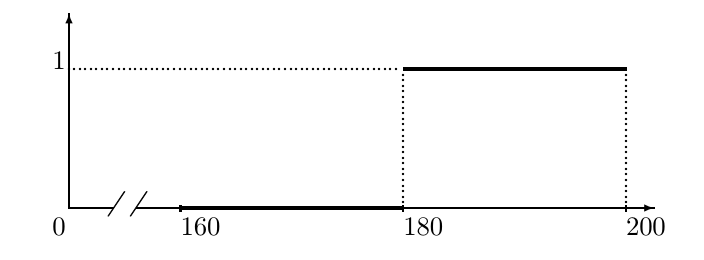
\includegraphics[width=100mm]{Images/Fig1.png}
	\vspace{-0.5cm}
	\caption{تابع عضویت افراد قد بلند در مجموعه‌های کلاسیک}\label{fig:f_1}
\end{figure}
حال همین مثال را در مجموعه‌های فازی تعریف می‌کنیم.  مجموعه‌ی فازی 
$B = \{ x,\mu_{B}(x) \}$
را در نظر بگیرید طوری که $x$ در بازه‌ی $[160,200]$ قرار دارد و تابع عضویت 
$\mu_{B}(x)$
بصورت زیر تعریف می‌شود:
$$
\mu_{B}(x)=\left \{
{
	  \frac{1}{2(30)^2}(x-140)^2
	  \atop
	  -\frac{1}{2(30)^2}(x-200)^2+1
}
\hskip 0.5cm
{
	if \hskip 0.5cm 160 \le x < 170,
	 \atop
   if \hskip 0.5cm  170 \le x \le 200.
} \right.
$$
تابع
$\mu_{B}(x)$
از نوع پیوسته قطعه به قطعه‌ی درجه دوم 
\LTRfootnote{continous piecewise-quadratic function}
می‌باشد. حال همانطور که در شکل 
\ref{fig:f_2}
نمودار این تابع نمایش داده است، اگر فردی دارای قد ۱۶۰ سانتی‌متر باشد مقدار کمی قد بلند (۰.۲۲ درجه) محسوب می‌شود و اگر قد شخصی ۱۸۰ سانتی‌متر باشد مقدار زیادی (۰.۷۸ درجه) قد بلند محسوب می‌شود. همچنین شخصی با قد ۲۰۰ سانتی‌متر کاملا قد بلند خواهد بود.
\cite{Bojadziev2007}
\begin{figure}[h]
\centering 
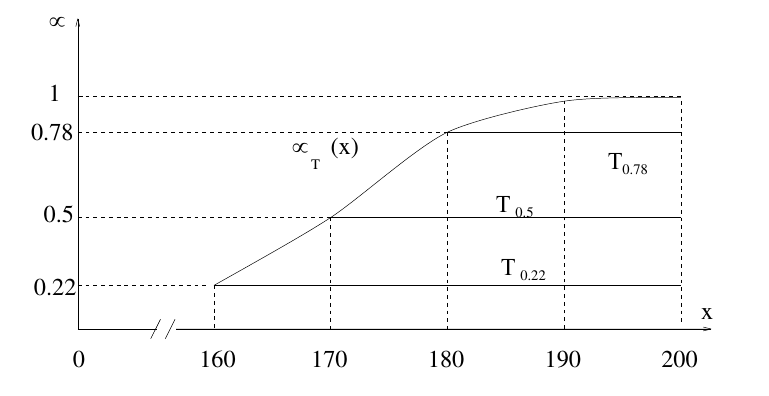
\includegraphics[width=100mm]{Images/Fig2.png}
\vspace{-0.5cm}
\caption{تابع عضویت افراد قد بلند در مجموعه‌‌های فازی}\label{fig:f_2}
\end{figure}
\end{exmp}
\begin{exmp}\label{ex:e_2}
\textbf{اعداد نزدیک به صفر:}
مجموعه‌ی $Z$ را مجموعه‌ی «اعداد نزدیک به صفر» در نظر بگیرید. آنگاه یک تابع عضویت ممکن برای این مجموعه به صورت زیر خواهد بود:
$$ 	\mu_{Z}(x)=e^{-x^2} $$
	طبق رابطه بالا اعداد صفر و ۲ به ترتیب با درجات عضویت
$e^0=1$
	و
$e^{-4}$
	 عضو مجموعه خواهند بود. همچنین ما می‌توانیم رابطه زیر
	 را نیز به عنوان تابع عضویت مجموعه‌ی اعداد نزدیک به صفر در نظر بگیریم:
$$
	 	\mu_{Z}(x)=\left \{
	 \begin{array}{ll}
		0 \hskip 0.5cm & 	 if \hskip 0.5cm  x < -1,\\
		x+1 \hskip 0.5cm & 	if \hskip 0.5cm -1 \le x < 0,\\
		1-x \hskip 0.5cm & 	 if \hskip 0.5cm 0 \le x < 1,\\
		0 \hskip 0.5cm & 	 if \hskip 0.5cm 1 \le x.
	 \end{array}
	  \right.
$$
	که در آن اعداد صفر و ۲ به ترتیب دارای درجات عضویت ۱ و صفر در این مجموعه هستند. نمودار این  دو تابع در ادامه آورده شده است. 
	\begin{figure}[b]
		\centering 
		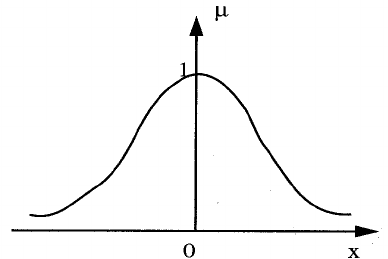
\includegraphics[width=75mm]{Images/Fig3.png}
		\vspace{-0.5cm}
		\caption{یک تابع عضویت ممکن برای مجموعه فازی «اعداد نزدیک به صفر»}\label{fig:f_3}
	\end{figure}
طبق این مثال برای هر مجموعه‌ی فازی می‌توان توابع عضویت متفاوتی را در نظر گرفت. کلماتی که یک مجموعه فازی را تعریف می‌کنند، خود نیز فازی هستند. به عنوان مثال اعداد نزدیک به صفر، تعریف دقیقی را ارائه نمی‌کند و به همین دلیل می‌توان توابع عضویت متفاوتی را برای تعریف توضیح ارائه شده برای این مجموعه در نظر گرفت. البته این نکته را نیز باید بخاطر داشت که توابع عضویت فازی نیستند و آنها یک تابع ریاضی دقیق هستند. 
 بنابراین همانطور که در این مثال نشان داده شد، یک توضیح فازی ارائه شد و توسط توابع عضویت، به غیرفازی  تبدیل شدند. در برخی مواقع این ابهام وجود دارد که نظریه مجموعه‌های فازی برای این است که همه مسائل را فازی کند، اما خواهیم دید که در مقابل مجموعه‌های فازی برای غیرفازی کردن مسائل استفاده خواهد شد.
\cite{Wang1997}	
\begin{figure}[h]
	\centering 
	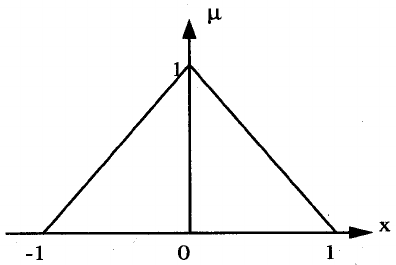
\includegraphics[width=75mm]{Images/Fig4.png}
	\vspace{-0.3cm}
	\caption{یک تابع عضویت دیگر برای مجموعه فازی «اعداد نزدیک به صفر»}\label{fig:f_4}
\end{figure}
\end{exmp}

%##################################################################
 \subsection{ مفاهیم پایه مجموعه‌های فازی}
\paragraph{پشتیبان}
 پشتیبان مجموعه‌ی فازی $A$، مجموعه‌ای قطعی است که شامل همه‌ی اعضایی از $A$ است که دارای درجه عضویت بزرگتر از صفر هستند.
 \begin{equation}\label{eq:e_supp}
 	Supp(A)=\{ x \in U\ |\ \mu_{A}(x) > 0 \}
\end{equation}
\paragraph{مجموعه فازی تهی}
اگر پشتیبان یک مجموعه‌ی فازی تهی باشد، آنگاه آن مجموعه‌ی فازی نیز تهی است. 
\paragraph{مجموعه‌ فازی منفرد}
مجموعه‌ی فازی که پشتیبان آن تنها یک عضو دارد را مجموعه‌ی فازی منفرد
\LTRfootnote{Fuzzy Singleton}
 گویند.
\paragraph{مرکز مجموعه فازی}
اگر مقدار میانگین تمام نقاطی که در آنها تابع عضویت مقدار ماکزیمم دارد، محدود باشد، در این صورت این مقدار میانگین مرکز مجموعه‌ی فازی می‌باشد. اگر مقدار میانگین مثبت بی‌نهایت (منفی بی‌نهایت) باشد، در این صورت مرکز مجموعه، کوچکترین (بزرگترین) نقطه‌ای است که در آن تابع عضویت به حداکثر مقدار خود می‌رسد. در شکل 
\ref{fig:f_5}
مرکز چندین مجموعه نمایش داده شده است.
\begin{figure}[h]
	\centering 
	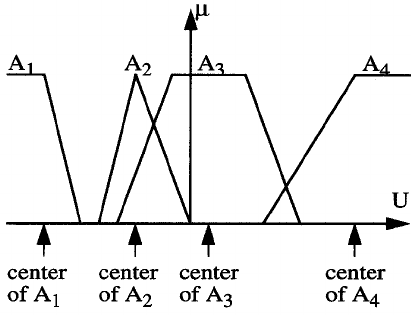
\includegraphics[width=75mm]{Images/Fig5.png}
	\vspace{-0.5cm}
	\caption{مرکز چند مجموعه‌ی فازی متداول}\label{fig:f_5}
\end{figure}
\paragraph{نقطه تقاطع}
نقطه‌ی گذر یا تقاطع 
\LTRfootnote{Crossover Point}
مجموعه‌ی فازی $A$ نقطه‌ای در مجموعه‌ی $U$ است که ارزش عضویت آن در مجموعه‌ی $A$ برابر ۰.۵ باشد.
\paragraph{ارتفاع}
ارتفاع یک مجموعه فازی برابر است با بزرگترین درجه عضویت اعضای آن مجموعه.
\paragraph{مجموعه فازی نرمال}
اگر ارتفاع یک مجموعه فازی برابر یک باشد، آن مجموعه فازی نرمال است. در شکل 
\ref{fig:f_6}
مجموعه‌ی فازی نرمال و غیرنرمال نمایش داده شده است.
\begin{figure}[h]
	\centering 
	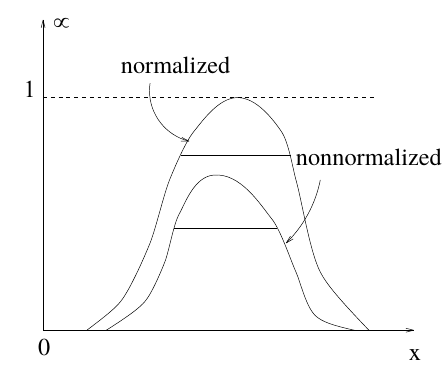
\includegraphics[width=75mm]{Images/Fig6.png}
		\vspace{-0.5cm}
	\caption{مجموعه فازی نرمال و غیرنرمال}\label{fig:f_6}
\end{figure}
\paragraph{نرمال سازی مجموعه فازی}
در صورتی که 
$ {\rm max}\ \mu_{A}(x) < 1$
باشد، آنگاه مجموعه $A$ غیرنرمال است. برای نرمال سازی این مجموعه کافیست طبق رابطه 
\ref{eq:e_normalize}
درجه عضویت همه‌ی اعضا را بر ماکزیمم درجه عضویت آن مجموعه تقسیم کنیم.
\begin{equation}\label{eq:e_normalize}
	\mu_{A}(x) \over {{\rm max}\ \mu_{A}(x)}
\end{equation}
\paragraph{برش $\alpha$}
یک برش آلفای 
\LTRfootnote{$\alpha$-cut}
مجموعه‌ فازی $A$ برابر است با مجموعه‌ای قطعی که در آن اعضا با درجه عضویت بزرگتر و یا مساوی $\alpha$ قرار دارند. مقدار $\alpha$ می‌تواند در بازه‌ی 
$[0,1]$
باشد. 
\begin{equation}\label{eq:e_acut}
	A_{\alpha}=\{ x \in U |\ \mu_{A}(x) \ge \alpha \}, \alpha \in [0,1]
\end{equation}
\paragraph{برش $\alpha$ قوی}
اگر رابطه‌ی 
\ref{eq:e_acut}
را به صورت زیر تعریف کنیم، آنگاه یک برش آلفای قوی خواهیم داشت. یعنی همانند برش آلفا ولی با این تفاوت که اعضای با درجه عضویت مساوی $\alpha$ را در نظر نگیریم.
\begin{equation}\label{eq:e_acuta}
A_{\alpha}=\{ x \in U |\ \mu_{A}(x) > \alpha \}, \alpha \in [0,1]
\end{equation}
\textbf{نکته:}
در برش آلفای قوی، اگر $\alpha$ را برابر با صفر در نظر بگیریم مجموعه‌ی پشتیبان بدست خواهد آمد.
\paragraph{مجموعه فازی محدب}
مجموعه فازی $A$ را در $R^n$ محدب
\LTRfootnote{Convex Fuzzy Set}
 گویند، اگر و تنها اگر:
\begin{equation}\label{eq:e_covset}
\mu_A\ [\lambda x_1+(1-\lambda)x_2] \ge min\ [ \mu_{A}(x_1), \mu_{A}(x_2) ]
\end{equation} 
برای همه‌ی
 $x_1,x_2 \in R^n$
 و همه‌ی
 $\lambda \in [0,1]$.\\
 به طور شهودی مجموعه‌ی $A$ در صورتی محدب خواهد بود که شکل آن دارای دره نباشد. به عبارت دیگر مجموعه می‌تواند صعود کند و سپس نزول کند، ولی دیگر اجازه صعود ندارد. مثالی از این مجموعه‌ها در شکل 
 \ref{fig:f_convset}
 نشان داده شده است.
\begin{figure}[h]
	\centering 
	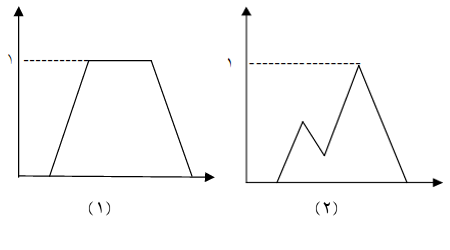
\includegraphics[width=75mm]{Images/Fig7.png}
	\vspace{-1cm}
	\caption{(۱) مجموعه‌ فازی محدب (۲) مجموعه فازی غیرمحدب}\label{fig:f_convset}
\end{figure}
\paragraph{کاردینالیتی}
کاردینالیتی
\LTRfootnote{Cardinality}
 یا عدد اصلی یک مجموعه برابر است با مجموع درجات عضویت اعضای آن:
\begin{equation}\label{eq:e_cardinality}
	|A|=\sum_{i} \mu_{A}(x_i)
\end{equation}
 %*********************************************************************
 \subsection{ روابط بین مجموعه‌های فازی}
 همانند آنچه که در جدول
 \ref{table:t_classic_rel}
 برای روابط بین مجموعه‌های کلاسیک مطرح شد، برای مجموعه‌های فازی نیز در ادامه تعریف خواهند شد.
 فرض کنید دو مجموعه‌ی $A$ و $B$ در مجموعه‌ی جهانی $U$ به صورت زیر باشد:
$$
A = \{ (x, \mu_{A}(x)) \}, \mu_{A}(x) \in [0,1], \atop
B = \{ (x, \mu_{B}(x)) \}, \mu_{B}(x) \in [0,1].
$$ 
تعریف روابط بین این دو مجموعه در ادامه آورده شده است.
 \paragraph{تساوی}
دو مجموعه‌ی فازی $A$ و $B$ مساوی خواهند بود ($A=B$)، اگر و تنها اگر رابطه زیر برقرار باشد:
\begin{equation}\label{eq:e_fset_rel_eq}
 \mu_{A}(x) = \mu_{B}(x)\  {\rm for\ all}\ x\in U
\end{equation}
\paragraph{زیرمجموعه}
مجموعه‌ی فازی $A$ زیرمجموعه‌ی $B$ خواهد بود ($A \subseteq B$)، اگر و تنها اگر رابطه زیر برقرار باشد:
\begin{equation}\label{eq:e_fset_rel_subseteq}
\mu_{A}(x) \le \mu_{B}(x)\  {\rm for\ all}\ x\in U
\end{equation}
\paragraph{زیرمجموعه سره}
مجموعه‌ی فازی $A$ زیرمجموعه‌ی سره $B$ خواهد بود ($A \subset B$)، اگر مجموعه‌ی $A$ زیر مجموعه‌ی $B$ باشد ولی این دو مجموعه با یکدیگر مساوی نباشند. این رابطه به صورت زیر تعریف می‌شود:
\begin{equation}\label{eq:e_fset_rel_subset}
\left\{ \begin{array}{ll} 
\mu_{A}(x) \le \mu_{B}(x) &    {\rm for\ every}\ x \in U, \\
\mu_{A}(x) < \mu_{B}(x) &  {\rm for\ at\ least\ one}\ x \in U.
\end{array} \right.
\end{equation}
 %*********************************************************************
 \subsection{عملیات بر روی مجموعه‌های فازی}
 مجموعه‌های فازی $A$ و $B$ را در مجموعه‌ی جهانی $U$ در نظر بگیرید. عملیات مکمل، اشتراک و اجتماع برای این مجموعه‌ها در ادامه تعریف شده است.
\paragraph{اجتماع}
 اجتماع دو مجموعه‌ی $A$ و $B$ برابر است با ماکزیمم درجه عضویت $x \in U$ در $A$ و $B$:
 \begin{equation}\label{eq:e_fset_op_union}
 \mu_{A \cup B}(x) = {\rm Max}\ [\mu_{A}(x), \mu_{B}(x)]
 \end{equation}
\paragraph{ اشتراک}
اشتراک دو مجموعه‌ی $A$ و $B$ برابر است با می‌نیمم درجه عضویت $x \in U$ در $A$ و $B$:
 \begin{equation}\label{eq:e_fset_op_intersect}
 \mu_{A \cap B}(x) = {\rm Min}\ [\mu_{A}(x), \mu_{B}(x)]
 \end{equation}
 \paragraph{ مکمل}
 مکمل مجموعه‌ی $A$ برابر است با تفاضل درجه عضویت $x \in U$ در $A$ از ماکزیمم درجه عضویت یعنی ۱:
 \begin{equation}\label{eq:e_fset_op_complement}
 \mu_{\overline{A}}(x) = 1- \mu_{A}(x)
 \end{equation}
 \paragraph{تفاضل}
 تفاضل مجموعه‌ی $A$ و $B$ برابر است با اشتراک مجموعه‌ی $A$ و مجموعه‌ی مکمل $B$:
 \begin{equation}\label{eq:e_fset_op_difference}
 \mu_{A|B}(x) = \mu_{A \cap \overline{B}}(x) = \mu_{A}(x) \cap [ 1 - \mu_{B}(x)]
 \end{equation}
\begin{exmp}
	فرض کنید دو مجموعه‌ی $A$ و $B$ به صورت زیر باشند:
\begin{figure}[h]
	\centering 
	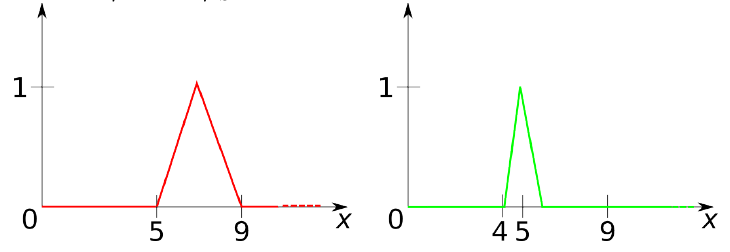
\includegraphics[width=100mm]{Images/Fig8.png}
	\vspace{-0.5cm}
	\caption{دو مجموعه‌ی فازی $ A $ و $ B $} \label{fig:f_fset_op_exmp}
\end{figure}\\
تعریف اجتماع، اشتراک و مکمل برای این مجموعه‌ها بر روی نمودار، در ادامه آورده شده است. 
\begin{figure}[h]
	\centering 
	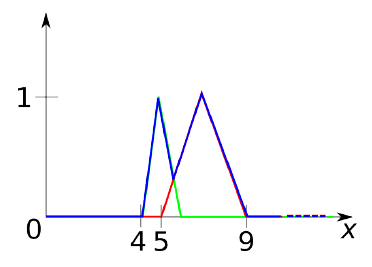
\includegraphics[width=75mm]{Images/Fig9.png}
	\vspace{-0.5cm}
	\caption{اجتماع دو مجموعه‌ی فازی $ A $ و $ B $} \label{fig:f_fset_op_exmp_union}
\end{figure}
\begin{figure}[h]
	\centering 
	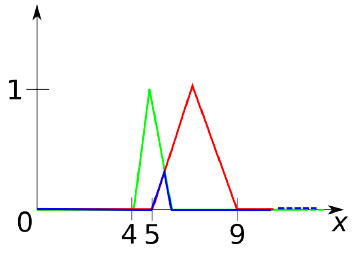
\includegraphics[width=75mm]{Images/Fig10.png}
	\vspace{-0.5cm}
	\caption{اشتراک دو مجموعه‌ی فازی $ A $ و $ B $} \label{fig:f_fset_op_exmp_intersect}
\end{figure}
\begin{figure}[h]
	\centering 
	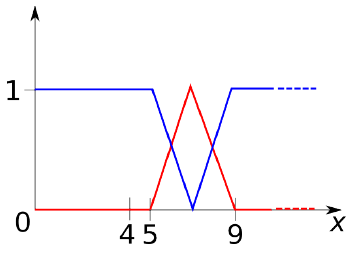
\includegraphics[width=75mm]{Images/Fig11.png}
	\vspace{-0.5cm}
	\caption{مکمل مجموعه‌ی فازی $A$} \label{fig:f_fset_op_exmp_complement}
\end{figure}\cite{Spada}\\
\end{exmp}


 \subsection{‌خواص عملیات در مجموعه‌های فازی}
همه‌ی خواصی که برای مجموعه‌های کلاسیک در جدول 
\ref{table:t_classic_properties}
آورده شد، به جز «قوانین متمم» برای مجموعه‌های فازی نیز صادق هستند. 
قوانین متمم در مجموعه های کلاسیک به صورت 
$
A \cap \overline{A} = \varnothing {\rm \ And}\ A \cup \overline{A} = U $
تعریف می‌شوند. این قوانین توسط نمودار ون نیز در شکل 
\ref{fig:f_fset_excludedmiddle_classic}
نشان داده شده‌اند. 
\begin{figure}[!htbp]
	\centering 
	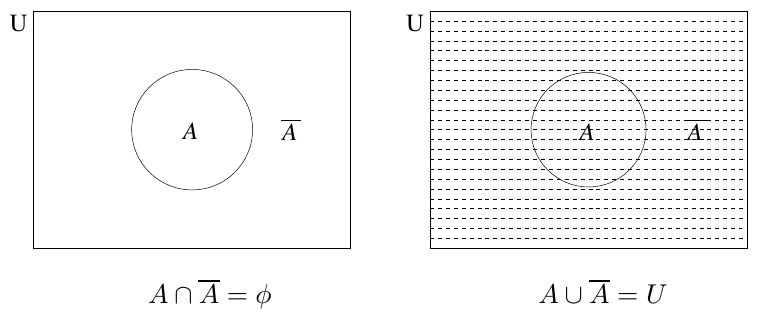
\includegraphics[width=75mm]{Images/Fig12.png}
	\vspace{-0.5cm}
	\caption{قوانین متمم برای مجموعه‌های کلاسیک} \label{fig:f_fset_excludedmiddle_classic}
\end{figure}\\
واضح است در مجموعه‌های فازی این قانون معتبر نمی‌باشد. نبود این قانون در مجموعه‌های فازی باعث می‌شود که آنها نسبت به مجموعه‌های کلاسیک دقت کمتری داشته باشند ولی این موضوع باعث انعطاف‌پذیری بیشتر مجموعه‌های فازی می‌شود و باعث می‌شود مجموعه‌های فازی برای توصیف ابهام و فرایندهای حاوی اطلاعات ناقص، مناسب باشند.
\begin{figure}[h]
	\centering 
	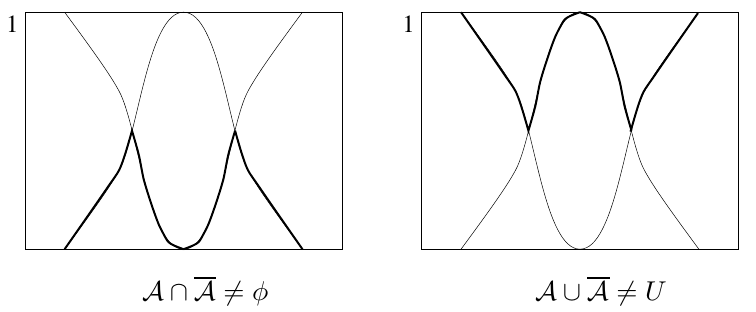
\includegraphics[width=75mm]{Images/Fig13.png}
	\vspace{-0.5cm}
	\caption{عدم اعتبار قانون متمم برای مجموعه‌های فازی} \label{fig:f_fset_excludedmiddle_fuzzy}
\end{figure}\cite{Bojadziev2007} 
 \subsection{‌توابع عضویت} 
 نحوه ایجاد مجموعه‌های فازی و تعریف تابع عضویت آنها بستگی به زمینه و دامنه کاربری آنها دارد. تعریف یک مجموعه فازی برای مفهوم مورد نظر با تعریف یک تابع عضویت مناسب برای آن کامل می‌شود. تعریف تابع عضویت مناسب بسیار مهم است؛ زیرا اگر تابع عضویت تعریف شده برای مجموعه فازی مناسب نباشد، کلیه تحلیل‌ها و بررسی‌ها پس از آن دچار انحراف می‌شوند. در ادامه چندین تابع عضویت متداول در مجموعه‌های فازی آورده شده است.
 \paragraph{تابع عضویت مثلثی}
 تابع عضویت مثلثی
 \LTRfootnote{Triangular}
  با سه پارامتر تعریف می‌شود که به شرح ذیل است:
 \begin{equation}\label{eq:e_fset_memfunc_triangle}
 triangle (x: a, m, b) = \left\{ 
 \begin{array}{ll}
 0 &  x < a, \\ \vspace{0.3cm}
\mathlarger{\frac{x-a}{m-a}} & a \leq x \leq m, \\ 
\mathlarger{ \frac{b-x}{b-m}} & m \leq x \leq b, \\
 0 & x > b.
 \end{array}
 \right.
 \end{equation}
پارامترهای $a$ و $b$، به ترتیب ابتدا و انتهای بازه هستند و پارامتر $m$ بیانگر رأس مثلث می‌باشد.(شکل \ref{fig:f_14})
\cite{Pedrycz2007}
\begin{figure}[h]
	\centering 
	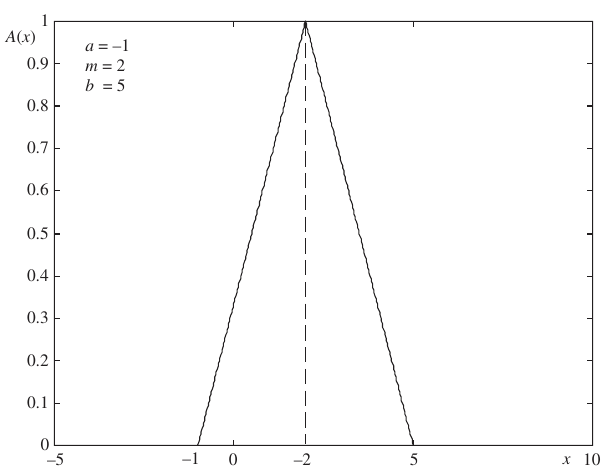
\includegraphics[width=75mm]{Images/Fig14.png}
	\vspace{-0.5cm}
	\caption{نمونه‌ای از تابع عضویت مثلثی}\label{fig:f_14}
\end{figure}
\paragraph{تابع عضویت ذوزنقه‌ای}
تابع عضویت ذوزنقه‌ای
\LTRfootnote{Trapezoidal}،
 نوعی تابع خطی قطعه به قطعه است که با ۴ پارامتر $(a, m, n, b)$ تعریف می‌شود. هر یک از این پارامترها، یکی از چهار قسمت تابع عضویت را مشخص می‌کنند. تعریف این تابع به شرح ذیل است:
\begin{equation}\label{eq:e_fset_memfunc_trapezoidal}
trapezoidal (x: a, m, n, b) = \left\{ 
\begin{array}{cl}
0 &  x \leq a, \\ 
\mathlarger{\frac{x-a}{m-a}} & a<x<m, \\ 
1 & m \leq x \leq n, \\
\mathlarger{ \frac{b-x}{b-n}} & n<x<b, \\
0 & x \geq b.
\end{array}
\right.
\end{equation}
پارامترهای $a$ و $b$، به ترتیب ابتدا و انتهای بازه هستند و پارامترهای $m$ و $n$، بیانگر قسمت هم سطح تابع می‌باشند.(شکل \ref{fig:f_15})
\cite{Pedrycz2007}
\begin{figure}[h]
	\centering 
	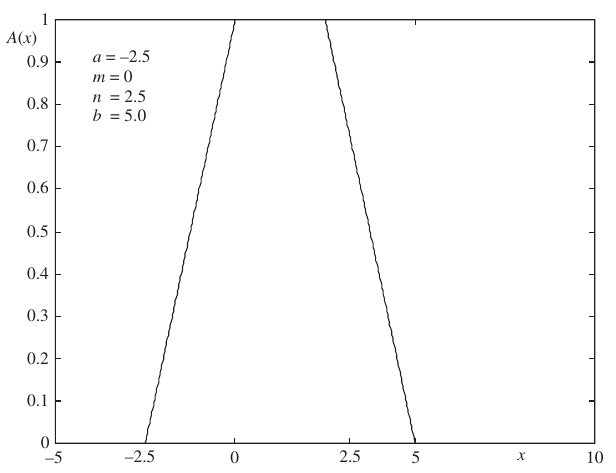
\includegraphics[width=75mm]{Images/Fig15.png}
	\vspace{-0.5cm}
	\caption{نمونه‌ای از تابع عضویت ذوزنقه‌ای}\label{fig:f_15}
\end{figure}
\paragraph{تابع عضویت گوسی}
تابع عضویت گوسی
\LTRfootnote{Gaussian}،
 با استفاده از دو پارامتر $(a, \sigma)$ تعریف می‌شود. این تابع به شرح ذیل است:
\begin{equation}\label{eq:e_fset_memfunc_gausi}
gaussian (x: a, \sigma) = \exp \left( - \frac{(x-m)^2}{\sigma^2} \right)
\end{equation}
پارامتر $a$، نقطه‌ی رأس تابع و $\sigma$ میزان پهنای تابع عضویت را مشخص می‌کند. مقادیر بالاتر $\sigma$، باعث گستره‌ی بیشتر تابع عضویت می‌شود.(شکل \ref{fig:f_16})
\cite{Pedrycz2007}
\begin{figure}[h]
	\centering 
	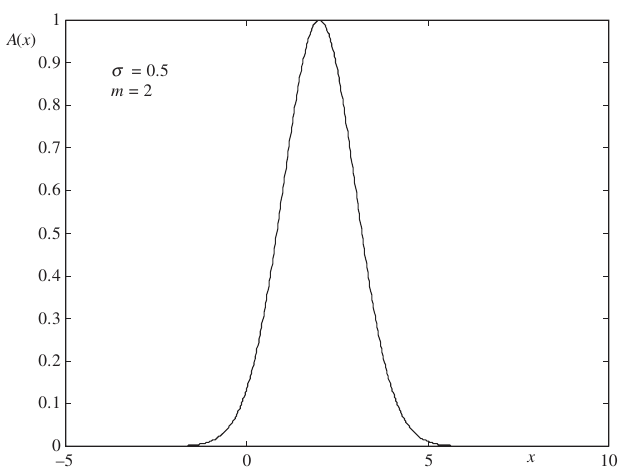
\includegraphics[width=75mm]{Images/Fig16.png}
	\vspace{-0.5cm}
	\caption{نمونه‌ای از تابع عضویت گوسی}\label{fig:f_16}
\end{figure}
\paragraph{تابع عضویت زنگوله‌ای}
تابع عضویت زنگوله‌ای
\LTRfootnote{Bell Shape}،
با استفاده از سه پارامتر $(a, b, c)$ تعریف می‌شود. این تابع به شرح ذیل است:
\begin{equation}\label{eq:e_fset_memfunc_bellshape}
bell\ shape (x: a, b, c) = \frac{1}{1+ \mathlarger{ \left| \frac{x-c}{a}\right| ^{2b}} }
\end{equation}
پارامتر $c$، مرکز تابع عضویت را نشان می‌دهد. همچنین پارامتر $b$، شیب و پارامتر $a$ پهنای تابع را مشخص می‌کند.(شکل \ref{fig:f_17})
 \\
\begin{figure}[h]
	\centering 
	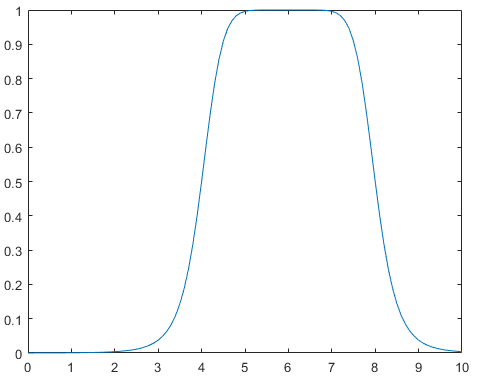
\includegraphics[width=75mm]{Images/Fig17.png}
	\vspace{-0.5cm}
	\caption{نمونه‌ای از تابع عضویت زنگوله‌ای}\label{fig:f_17}
\end{figure}
در شکل 
\ref{fig:f_20}
نیز تغییرات پارامترهای تابع و نحوه‌ی تاثیر آنها نشان داده شده است. 
\cite{yen1999fuzzy}
\begin{figure}[!htbp]
	\centering 
	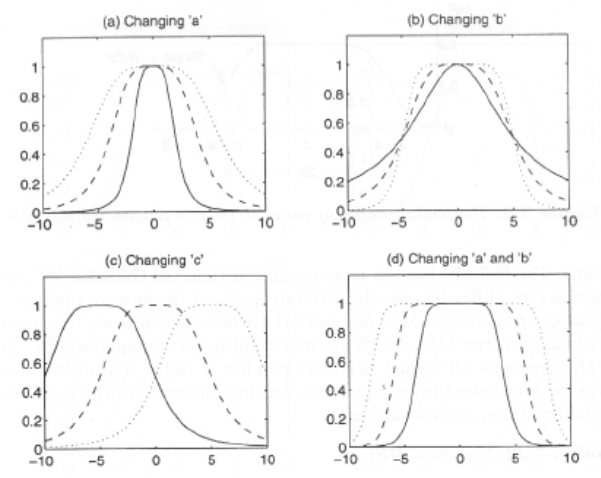
\includegraphics[width=100mm]{Images/Fig20.png}
	\vspace{-0.5cm}
	\caption{تغییر پارامترهای تابع زنگوله‌ای و نحوه تاثیر آنها بر تابع}\label{fig:f_20}
\end{figure}
\paragraph{تابع عضویت سیگمویدال}
تابع عضویت سیگمویدال
\LTRfootnote{Sigmoidal}،
با استفاده از دو پارامتر $(a, c)$ تعریف می‌شود. این تابع به شرح ذیل است:
\begin{equation}\label{eq:e_fset_memfunc_sigmoidal}
sigmoidal (x: a, c) = \frac{1}{1+\mathlarger{e^{-a(x-c)}}} 
	\end{equation}
	پارامتر $a$، شیب و پارامتر $c$، مرکز تابع را مشخص می‌کند.(شکل \ref{fig:f_18})
\cite{yen1999fuzzy}
	\begin{figure}[h]
		\centering 
		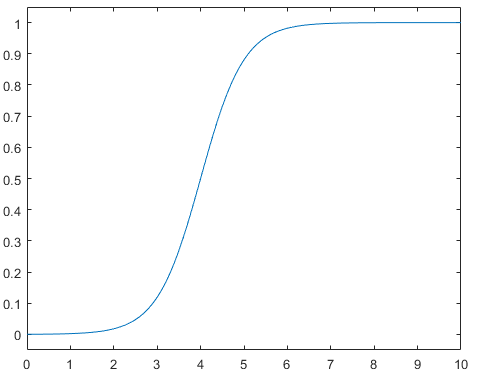
\includegraphics[width=75mm]{Images/Fig18.png}
		\vspace{-0.5cm}
		\caption{نمونه‌ای از تابع عضویت سیگمویدال}\label{fig:f_18}
	\end{figure}
%**************************************************************************
 \subsection{‌اعداد فازی} 
 اگر یک مجموعه‌ی فازی \textit{محدب} و \textit{نرمال} باشد و تابع عضویت آن در 
 $\Re$
 تعریف شود، به آن عدد فازی گویند. بنابراین عدد فازی (مجموعه فازی)، بازه‌ی عددی حقیقی را نشان می‌دهد که ابتدا و انتهای بازه، فازی هستند.
 \cite{Lee2005}
  اعداد فازی برای توصیف غیر دقیق اعداد استفاده می‌شوند. 
  به عنوان مثال در شکل 
 \ref{fig:f_convset}
 مجموعه‌ی (a) عدد فازی است و مجموعه‌ی (b) نیست.
 %***********************************************************************
  \subsection{‌متغیرهای کلامی}
  مفهوم اعداد فازی، نقش مهمی در فرموله کردن کمی متغیرهای فازی دارند. اعداد فازی می‌توانند بیانگر مفاهیم کلامی مانند خیلی کوچک، کوچک، متوسط و... باشند. بدین ترتیب می‌توان با استفاده از اعداد فازی متغیرهای کلامی
  \LTRfootnote{Linguistic Variable}
   را ایجاد کرد. \\
   هر متغیر کلامی شامل حالت‌هایی است که توسط عبارات کلامی
   \LTRfootnote{Linguistic Terms}
   بیان می‌شوند. هریک از این عبارات، عددی فازی هستند که بر پایه‌ی آن متغیر، در بازه‌ای مشخص تعریف می‌شوند و مقادیر تقریبی از متغیر کلامی را نشان می‌دهند. \\
   مثالی از متغیر کلامی در شکل
   \ref{fig:f_19}
   آورده شده است. در این مثال، «عملکرد»
   \LTRfootnote{Performance}
   متغیری کلامی است که توسط عبارات کلامی «خیلی کم، کم، متوسط، زیاد، خیلی زیاد» تعریف شده است. این عبارات هر کدام توسط عددی فازی مشخص شده‌اند. تابع عضویت این مجموعه‌های فازی، یک تابع ذوزنقه‌ای در نظر گرفته شده است. بازه‌ی متغیر کلامی نیز $[1, 100]$ می‌باشد. 
     \cite{Klir1995}
   \\
   به عنوان مثال اگر میزان عملکرد (انسان، ماشین، سازمان، روش و...)، برابر ۸۳.۷۵ باشد، با درجه عضویت ۰.۵ به مجموعه‌ی «عملکرد خیلی زیاد» و با درجه‌ عضویت ۰.۵ به مجموعه‌ی «عملکرد زیاد» تعلق دارد. همچنین این میزان عملکرد نه متوسط است، نه کم و نه خیلی کم. 

  	\begin{figure}[h]
  	\centering 
  	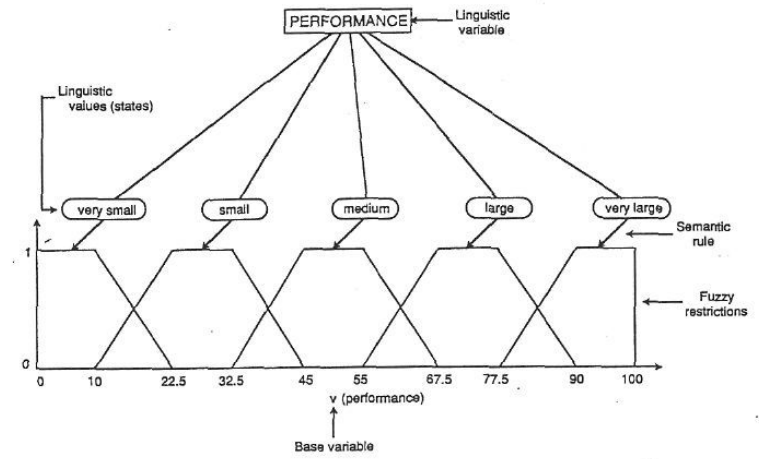
\includegraphics[width=125mm]{Images/Fig19.png}
  	\vspace{-0.5cm}
  	\caption{مثالی از متغیرهای کلامی}\label{fig:f_19}
  \end{figure}
 \subsection{رابطه‌های فازی}
 \subsection{عملیات بر روی رابطه‌های فازی}